\documentclass{standalone}
\usepackage{tikz}
\usepackage{pgfplots}
\pgfplotsset{compat=1.12,width=7cm}%
\begin{document}
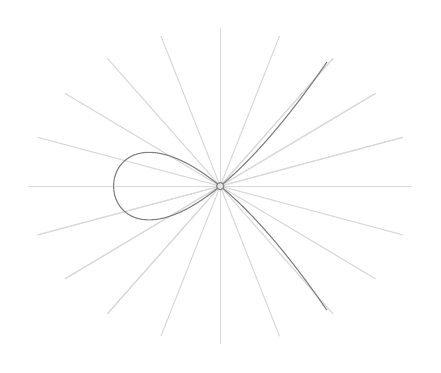
\begin{tikzpicture}
\begin{axis}[hide axis,xmin=-2,xmax=2,ymin=-2,ymax=2]
\newcommand{\RRR}{1.8}
\newcommand{\lineclr}{gray!30}
\draw[\lineclr] 
	({\RRR*cos(3.1415*0/10 r)},{\RRR*sin(3.1415*0/10 r)}) 
-- ({-\RRR*cos(3.1415*0/10 r)},{-\RRR*sin(3.1415*0/10 r)});
\draw[\lineclr] 
	({\RRR*cos(3.1415*1/10 r)},{\RRR*sin(3.1415*1/10 r)}) 
-- ({-\RRR*cos(3.1415*1/10 r)},{-\RRR*sin(3.1415*1/10 r)});
\draw[\lineclr] 
	({\RRR*cos(3.1415*2/10 r)},{\RRR*sin(3.1415*2/10 r)}) 
-- ({-\RRR*cos(3.1415*2/10 r)},{-\RRR*sin(3.1415*2/10 r)});
\draw[\lineclr] 
	({\RRR*cos(3.1415*3/10 r)},{\RRR*sin(3.1415*3/10 r)}) 
-- ({-\RRR*cos(3.1415*3/10 r)},{-\RRR*sin(3.1415*3/10 r)});
\draw[\lineclr] 
	({\RRR*cos(3.1415*4/10 r)},{\RRR*sin(3.1415*4/10 r)}) 
-- ({-\RRR*cos(3.1415*4/10 r)},{-\RRR*sin(3.1415*4/10 r)});
\draw[\lineclr] 
	({\RRR*cos(3.1415*1/10 r)},{-\RRR*sin(3.1415*1/10 r)}) 
-- ({-\RRR*cos(3.1415*1/10 r)},{\RRR*sin(3.1415*1/10 r)});
\draw[\lineclr] 
	({\RRR*cos(3.1415*2/10 r)},{-\RRR*sin(3.1415*2/10 r)}) 
-- ({-\RRR*cos(3.1415*2/10 r)},{\RRR*sin(3.1415*2/10 r)});
\draw[\lineclr] 
	({\RRR*cos(3.1415*3/10 r)},{-\RRR*sin(3.1415*3/10 r)}) 
-- ({-\RRR*cos(3.1415*3/10 r)},{\RRR*sin(3.1415*3/10 r)});
\draw[\lineclr] 
	({\RRR*cos(3.1415*4/10 r)},{-\RRR*sin(3.1415*4/10 r)}) 
-- ({-\RRR*cos(3.1415*4/10 r)},{\RRR*sin(3.1415*4/10 r)});
\draw[\lineclr] 
	({\RRR*cos(3.1415*1/10 r)},{\RRR*sin(3.1415*1/10 r)}) 
-- ({-\RRR*cos(3.1415*1/10 r)},{-\RRR*sin(3.1415*1/10 r)});
\draw[\lineclr] 
	({\RRR*cos(3.1415*2/10 r)},{\RRR*sin(3.1415*2/10 r)}) 
-- ({-\RRR*cos(3.1415*2/10 r)},{-\RRR*sin(3.1415*2/10 r)});
\draw[\lineclr] 
	({\RRR*cos(3.1415*3/10 r)},{\RRR*sin(3.1415*3/10 r)}) 
-- ({-\RRR*cos(3.1415*3/10 r)},{-\RRR*sin(3.1415*3/10 r)});
\draw[\lineclr] 
	(0,\RRR) 
-- (0,{-\RRR});
\newcommand{\curveclr}{gray}
  \addplot[domain=-1:0,\curveclr,samples=200]{sqrt(x^2+x^3)};%
  \addplot[domain=-1:0,\curveclr,samples=200]{-sqrt(x^2+x^3)};%
  \addplot[domain=0:1,\curveclr]{sqrt(x^2+x^3)};%
  \addplot[domain=0:1,\curveclr]{-sqrt(x^2+x^3)};%
  \fill[gray!20,draw=gray] (axis cs:0,0) circle (1.3pt);
\end{axis}
\end{tikzpicture}
\end{document}
